\documentclass[tikz,border=3pt]{standalone}
\usepackage{amsmath}
\usepackage{MnSymbol}
\usetikzlibrary{arrows.meta,calc,fit}
\definecolor{accent}{RGB}{210,137,72}
\definecolor{join}{RGB}{170,170,170}
\newcommand{\Arr}{\operatorname{arr}}
\newcommand{\First}{\operatorname{first}}
\newcommand{\comp}{\mathrel{\textcolor{join}{\ggg}}}
\begin{document}
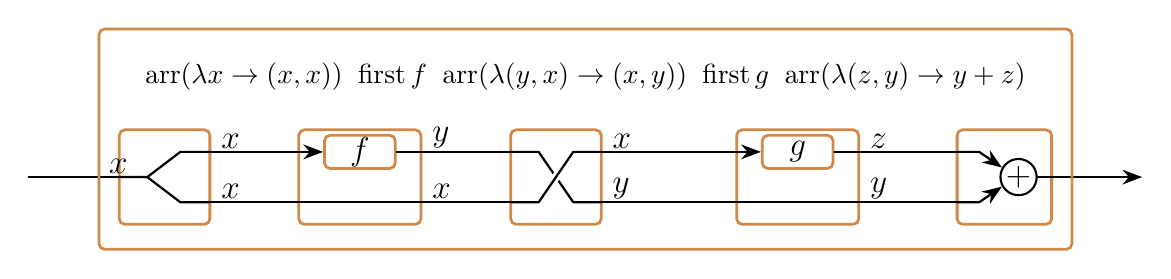
\begin{tikzpicture}[
  >={Stealth[length=2.5mm]},
  flow/.style={draw=black,line width=.8pt,line cap=round,line join=round},
  block/.style={draw=accent,rounded corners=2pt,line width=1pt},
  innerblock/.style={block,minimum width=.9cm,minimum height=.42cm,inner sep=0pt},
  lab/.style={anchor=south west,inner sep=.5pt},
  every node/.style={font=\large}
]
\def\u{.32}
\def\d{-.32}
\def\h{1.20}
\def\splitw{1.15}
\def\funw{1.55}
\def\swapw{1.15}
\def\addw{1.20}
\def\gapA{1.13}
\def\gapB{1.14}
\def\gapC{1.72}
\def\gapD{1.25}
\def\labx{.12}
\def\laby{.02}
\def\plusx{.18}
\def\turnx{-.32}
\tikzset{
pics/split/.style={code={
  \node[block,minimum width=\splitw cm,minimum height=\h cm,inner sep=0pt] (-box) at (0,0) {};
  \path ({-\splitw/2},0) coordinate (-in) ({\splitw/2},\u) coordinate (-up) ({\splitw/2},\d) coordinate (-down);
  \draw[flow] (-in)--(-.22,0)--(.20,\u)--(-up) (-.22,0)--(.20,\d)--(-down);
}},
pics/first/.style args={#1}{code={
  \node[block,minimum width=\funw cm,minimum height=\h cm,inner sep=0pt] (-box) at (0,0) {};
  \node[innerblock] (-fun) at (0,\u) {$#1$};
  \path ({-\funw/2},\u) coordinate (-iu) ({-\funw/2},\d) coordinate (-id) ({\funw/2},\u) coordinate (-ou) ({\funw/2},\d) coordinate (-od);
  \draw[flow,->] (-iu)--(-fun.west);
  \draw[flow] (-fun.east)--(-ou) (-id)--(-od);
}},
pics/swap/.style={code={
  \node[block,minimum width=\swapw cm,minimum height=\h cm,inner sep=0pt] (-box) at (0,0) {};
  \path ({-\swapw/2},\u) coordinate (-iu) ({-\swapw/2},\d) coordinate (-id) ({\swapw/2},\u) coordinate (-ou) ({\swapw/2},\d) coordinate (-od);
  \draw[flow] (-iu)--(-.22,\u)--(.22,\d)--(-od);
  \draw[white,line width=3pt,line cap=round] (-.07,-.10)--(.07,.10);
  \draw[flow] (-id)--(-.22,\d)--(.22,\u)--(-ou);
}},
pics/add/.style={code={
  \node[block,minimum width=\addw cm,minimum height=\h cm,inner sep=0pt] (-box) at (0,0) {};
  \node[draw=black,circle,line width=.75pt,minimum size=.46cm,inner sep=0pt] (-sum) at (\plusx,0) {$+$};
  \path ({-\addw/2},\u) coordinate (-iu) ({-\addw/2},\d) coordinate (-id) ({\addw/2},0) coordinate (-out);
  \draw[flow,->] (-iu)--(\turnx,\u)--(-sum.150);
  \draw[flow,->] (-id)--(\turnx,\d)--(-sum.210);
  \draw[flow] (-sum.east)--(-out);
}}}
\coordinate (copyc) at (0,0);
\coordinate (fc) at ($(copyc)+({(\splitw+\funw)/2+\gapA},0)$);
\coordinate (swapc) at ($(fc)+({(\funw+\swapw)/2+\gapB},0)$);
\coordinate (gc) at ($(swapc)+({(\swapw+\funw)/2+\gapC},0)$);
\coordinate (addc) at ($(gc)+({(\funw+\addw)/2+\gapD},0)$);
\pic (copy) at (copyc) {split}; \pic (f) at (fc) {first=f}; \pic (swap) at (swapc) {swap}; \pic (g) at (gc) {first=g}; \pic (add) at (addc) {add};
\coordinate (in) at ($(copy-in)+(-1.15,0)$); \coordinate (out) at ($(add-out)+(1.15,0)$);
\draw[flow] (in)--(copy-in) (copy-up)--(f-iu) (copy-down)--(f-id) (f-ou)--(swap-iu) (f-od)--(swap-id) (swap-ou)--(g-iu) (swap-od)--(g-id) (g-ou)--(add-iu) (g-od)--(add-id);
\draw[flow,->] (add-out)--(out);
\node[font=\normalsize] (title) at ($(in)!0.5!(out)+(0,1.28)$) {$\Arr(\lambda x\to(x,x))\comp\First f\comp\Arr(\lambda(y,x)\to(x,y))\comp\First g\comp\Arr(\lambda(z,y)\to y+z)$};
\node[block,fit=(title)(copy-box)(f-box)(swap-box)(g-box)(add-box),inner xsep=.24cm,inner ysep=.30cm] (outer) {};
\node[lab] at ($(outer.west |- copy-in)+(\labx,\laby)$) {$x$};
\foreach \p/\v in {copy-up/x,copy-down/x,f-ou/y,f-od/x,swap-ou/x,swap-od/y,g-ou/z,g-od/y}
  \node[lab] at ($(\p)+(\labx,\laby)$) {$\v$};
\end{tikzpicture}
\end{document}
